%%%%%%%%%%%%%%%%%%%%%%%%%%%%%%%%%%%%%%%%
% University Assignment Title Page
% LaTeX Template
% Version 1.0 (27/12/12)
%
% This template has been downloaded from:
% http://www.LaTeXTemplates.com
%
% Original author:
% WikiBooks (http://en.wikibooks.org/wiki/LaTeX/Title_Creation)
%
% License:
% CC BY-NC-SA 3.0 (http://creativecommons.org/licenses/by-nc-sa/3.0/)
%
% Instructions for using this template:
% This title page is capable of being compiled as is. This is not useful for
% including it in another document. To do this, you have two options:
%
% 1) Copy/paste everything between \begin{document} and \end{document}
% starting at \begin{titlepage} and paste this into another LaTeX file where you
% want your title page.
% OR
% 2) Remove everything outside the \begin{titlepage} and \end{titlepage} and
% move this file to the same directory as the LaTeX file you wish to add it to.
% Then add \input{./title_page_1.tex} to your LaTeX file where you want your
% title page.
%
%%%%%%%%%%%%%%%%%%%%%%%%%%%%%%%%%%%%%%%%%
%\title{Title page with logo}
%----------------------------------------------------------------------------------------
%	PACKAGES AND OTHER DOCUMENT CONFIGURATIONS
%----------------------------------------------------------------------------------------

\documentclass[11pt]{article}
\usepackage[utf8]{inputenc}
\usepackage{amsmath}
\usepackage{graphicx}
%\usepackage{lmodern}
\usepackage{hyperref}
\usepackage{tabularx}
\usepackage{amsmath}
\usepackage{float}
\usepackage[table]{xcolor}
\usepackage{booktabs}% http://ctan.org/pkg/booktabs

\usepackage{appendix}

\usepackage{fancyhdr}
\usepackage[hscale=0.76,vscale=0.76]{geometry} % Margin sizes
\usepackage{minted} % for this to work: `sudo apt install python-pygments` and use `-shell-escape` flag with `pdflatex`

\newcommand{\tabitem}{~~\llap{\textbullet}~~}
\newcommand{\HRule}{\rule{\linewidth}{0.5mm}} % Defines a new command for the horizontal lines, change thickness here

% To change the margin :)
\newenvironment{changemargin}[2]{%
\begin{list}{}{%
\setlength{\topsep}{0pt}%
\setlength{\leftmargin}{#1}%
\setlength{\rightmargin}{#2}%
\setlength{\listparindent}{\parindent}%
\setlength{\itemindent}{\parindent}%
\setlength{\parsep}{\parskip}%
}%
\item[]}{\end{list}}

\pagestyle{fancy}
\fancyhf{}
\rhead{Mission 2 -- Group G}
\lhead{\textit{LINGI2252}}
\cfoot{\thepage}

\begin{document}
    \begin{titlepage}
        \center % Center everything on the page

        %----------------------------------------------------------------------------------------
        %	HEADING SECTIONS
        %----------------------------------------------------------------------------------------

        \textsc{\LARGE Université Catholique de Louvain }\\[0.8cm] % Name of your university/college
        
\includegraphics[scale=0.45]{epl.jpg}
        \\[1.5cm]
        \textsc{\Large LINGI2252}\\[0.5cm] % Major heading such as course name
        \textsc{\large Software Maintenance and Evolution}\\[0.8cm] % Minor heading such as course title

        %----------------------------------------------------------------------------------------
        %	TITLE SECTION
        %----------------------------------------------------------------------------------------

        \HRule \\[0.4cm]
        { \huge \bfseries Mission 2: Improved prototype}\\[0.2cm] % Title of your document
        \HRule \\[1.5cm]

        %----------------------------------------------------------------------------------------
        %	AUTHOR SECTION
        %----------------------------------------------------------------------------------------

		\vfill
        \begin{minipage}{0.4\textwidth}
        \begin{flushleft} \large
        \emph{Authors:}\\
        \textbf{Group G}\\
        \textsc{Gustin}~Simon \\
        1171-14-00\\
        \textsc{Hallet}~Adrien \\
        3276-13-00\\
        \end{flushleft}
        \end{minipage}
        ~
        \begin{minipage}{0.4\textwidth}
        \begin{flushright} \large
        \emph{Professor:} \\
         \textsc{Mens}~Kim \\% Supervisor's Name
         \emph{Assistant:}\\
         \textsc{Duhoux}~Benoît
        \end{flushright}
        \end{minipage}\\[1cm]

        % If you don't want a supervisor, uncomment the two lines below and remove the section above
        %\Large \emph{Author:}\\
        %John~\textsc{Smith}\\[3cm] % Your name

        %----------------------------------------------------------------------------------------
        %	DATE SECTION
        %----------------------------------------------------------------------------------------

        {\large \today}\\[2cm] % Date, change the \today to a set date if you want to be precise

        %----------------------------------------------------------------------------------------
        %	LOGO SECTION
        %----------------------------------------------------------------------------------------

        % Include a department/university logo - this will require the graphicx package

        %----------------------------------------------------------------------------------------

        \vfill % Fill the rest of the page with whitespace
    \end{titlepage}

    \title{AAAAAA}
    \newpage

	\section{Introduction}
		For the course \textit{LINGI2252 -- Software Maintenance and Evolution}, we were asked to improve our first prototype of a house automation system. Specifically, we had to add a parametrization component which would allow us to specify the values and states of the variability points at execution time, a command line interpreter which would allow us to update the state of the house at run time and to use relevant design patterns to make the code more maintainable. We will discuss each of these extensions.

	\section{Parametrization component}
		The first extension we discuss is the parametrization component.
		It allows us to easily change the configuration of a house on two different executions without changing the code.
		It does this in a quite straightforward way: when the program executes, it starts by parsing a configuration file. It then creates a house that corresponds to the configuration described in this file.
		
		As can be expected, the design of this file has the same kind of structure as a house with a given configuration, that is a hierarchical structure. This structure is due to the fact that an automated house can be seen as a group of rooms (or floors, in our code \mintinline{java}{HousePart}s), which contain sensors, actuators and connected objects. This hierarchy can actually be seen on our class diagram: a \mintinline{java}{House} is made of \mintinline{java}{HousePart}s which contain \mintinline{java}{Controller}s.
		
		The configuration is contained within an external file formatted in \textit{JSON}. We chose this format for several reasons.
		First, it is well-known and heavily used as a format for configuration files. It is thus totally capable of handling this kind of task. If we had decided to make our own "configuration language", we could have very easily ended up with a syntax that would not fit all possible configurations perfectly, or with a flawed parser that would not work in certain cases.

		Secondly, the fact that it is a well-known format also means that parsers exist in most languages. We didn't have to implement one by ourselves or to use an incomplete or buggy implementation.

		Lastly, we are used to this format, which means we can work quickly and efficiently with it. The likelihood of us making an error while using it was thus smaller. This being said, using \textit{YAML} or \textit{TOML} would be perfectly legitimate choices, but we weren't as used to them as we are to \textit{JSON}. Note that using the latter instead of one of those two formats prevents us from having comments in our configuration files, which can be considered a problem.
		
		Notice that we didn't decide to implement the parser as a class of its own but rather to place the parsing logic inside the class \mintinline{java}{House}. As we use an external library to parse the configuration file, we figured out it wouldn't be very interesting to make a parser that would be only a couple of lines long. The configuration of the house is then done from within this class itself on basis of the parsed representation of the file. However, if we needed to parse files in other formats, making a class to handle the parsing would be a very good idea.
	
	\section{Command line interpreter}
		We discuss now the second extension we implemented, i.e. the command line interpreter. As we already said, this extension can be used to update the state of the house by typing commands during the execution of the program.
		
		Each command is quite simple to interpret with the first word corresponding to the action to execute and the following words being the (optional) parameter(s) of the action. We designed them this way in order to simplify the implementation of the interpreter: it simply test whether it recognizes the first word and calls a subsequent method accordingly, giving it the remaining words as arguments. This implementation is made in a class named \mintinline{java}{Scenario}. 
		
		A specificity of our implementation is also that commands can be received in two different ways: either sequentially from the standard input, or from an input file which contains one command per line. The behavior is then similar in both cases, the program interpreting and executing one command at a time in the order they are given.
		
		To make the code more reusable, we separated the interpretation of commands and the actions performed afterwards. Indeed, when a command is interpreted, the code calls a method that represents the action associated with this particular command. This improves reusability since it allows us to change the interpreter logic (for example, to create a different interpreter that would support another language or to add commands that would map to the same actions) and still be execute the exact same code for similar cases. It also makes our code easier to improve as adding a new command would be very easy. Finally, making it this way makes our code more readable.

  \section{Variability Points}
    \subsection{House Layout}
      The main variability point is the ability to adapt each possible house. Our application can modify the house layout via the parametrization component. Thanks to the \texttt{HousePart} component, we can split the \texttt{House} in as many subcomponents as we want (either one per floor, one per room, one per square meter, whatever fits the needs). The implementation is pretty straightforward as the \texttt{House} is nothing but a dynamic list of \texttt{HousePart}s.
      \begin{minted}[autogobble]{java}
        public class House{
          private static House instance;
          private static String filename;

          JSONObject config;
          ArrayList<HousePart> housePartList;
          ...
        }
      \end{minted}
      This list is produced from the configuration file which lists the rooms and their components, as you can see in the short following example.
      \begin{minted}[autogobble]{json}
      {
      "house": {
          "houseParts":[
              {
                  "name": "Entrance",
                  "accessible-houseParts": ["Kitchen"],
                  ...
                }
              ]
            }
          }
      \end{minted}

    \subsection{Controllers}
      In the configuration file, you can also modify the controllers (sensors, actuators and connected objects). You can place them and link a sensor to one or multiple actuators and/or connected objects. With such an implementation, you can link any kind of supported event (\emph{e.g.: detecting motion, smoke, humidity, ...}) to any kind of supported action (\emph{e.g.: opening a door, turning a light on, ...}). As for the house layout, this was done with a simple dynamic list of \texttt{Sensor}s linking to a dynamic list of \texttt{Actuator}s in a \texttt{HousePart}.
      \begin{minted}[autogobble]{java}
        HousePart(House parent, JSONObject housePart){
          ...
          if (housePart.has("actuators"))
              this.actuators = parseActuators(housePart.getJSONArray("actuators"));
          else
              this.actuators = new Actuator[0];
          if (housePart.has("objects"))
              this.connectedObjects = parseConnectedObjects(housePart.getJSONArray("objects"));
          else
              this.connectedObjects = new ConnectedObject[0];
          if (housePart.has("sensors"))
              this.sensorsJSON = housePart.getJSONArray("sensors");
          else
              this.sensors = new Sensor[0];
          ...
      \end{minted}

      Once again, the controllers' variability is handled by the JSON configuration file. Each \texttt{housePart} can only have one sensor of each type, but that does not reduce the system capacities. If you want to have two different motion sensors in the same room, you just have to declare two different house parts for this room.
      
      In the following example, you can see two declared sensors.
      The first one is a motion detector. When triggered, it sends a signal to the audio alarm in the kitchen, which will be triggered only if it is enabled.
      The second sensor is a smoke detector which triggers an audio alarm in the entrance. Note the broadcast parameter. It means that every actuator of the same type in the house will also be triggered.
      
      \begin{minted}[autogobble]{json}
      {"sensors": [
                    {
                        "type": "motion",
                        "actions": [{"housePart":"Kitchen", "actuator":"audio-alarm"}]
                    },
                    {
                        "type": "smoke",
                        "broadcast": true,
                        "actions": [{"housePart":"Entrance", "actuator":"audio-alarm"}]
                    }
                 ]}
      \end{minted}

    \subsection{Disable controllers}
      This one is self-explanatory. You can dynamically disable/enable controllers at runtime, effectively changing the observable behavior of the system. This is simply a clever use of boolean conditions modified by the running \texttt{Scenario} within the \texttt{HomeController}.
      \begin{minted}[autogobble]{java}
      public abstract class Controller {
        public String type;
        public double value = 0.0;
        private boolean enabled = true;
        private boolean inverted = false;
        ...
      }
      \end{minted}

    \subsection{Inverting controllers}
      Maybe you don't want an action to execute when a sensor is triggered, but when it is not. In the parametrization component, you can define an inverted sensor. This effectively doubles the possibilities as each sensor can now have two different behaviors. For example, you could want your door to close when the humidity sensor detects rain. Once again, the implementation is simple with a boolean condition checking if the \texttt{Sensor} is inverted.
      \begin{minted}[autogobble]{java}
      static void triggerActions(Sensor sensor){
          Actuator[] aList = sensor.getActuatorList();
          for(Actuator cActuator : aList){
              ...
              else { // Trigger one in given housePart
                  if (!sensor.isInverted())
                      cActuator.trigger();
                  else
                      cActuator.reset();
              }
          }
      }
      \end{minted}

    \subsection{Summary}
      In brief, we have two major parametrization types. The static parameters are loaded with the JSON file (\emph{e.g.: the house layout}), the dynamic parameters are real-time modifiable behaviors (\emph{e.g.: the controller (de)activation}).
      We have implemented 8 different possible actuators that can independently be enabled, 13 sensors types that can be disabled, inverted and broadcasted. This means that for each house part we can have $(8*2)*(13*2^3)=1664$ different possible combinations (some of them would of course be useless), leading to a huge amount of possibilities for the entire house.
      
      It is important to note that the JSON only serves as an initializer for the system. Therefore the entire configuration is accessible in real time and can be modified (we could then erase the old configuration with a new one for the next initialization). Implementing user commands to introduce even more parametrization would be easily done thanks to that and the used Design Patterns (see next).

  \section{Design Patterns}
    \subsection{Abstract Factory}
      We have three factories to create the controllers. \texttt{SensorFactory}, \texttt{ActuatorFactory} and \\ \texttt{ConnectedObjectFactory}. We do not have a higher-level factory because it would only reduce readability in the context. What motivated the use of this design pattern is that we had, by design, to parse the controllers from the parametrization component. This parsing was redundant in the code so we extracted the method. Extracting the creation of multiple objects that inherit from the same parent was done more easily with this factory pattern.
      \begin{figure}[!h]
        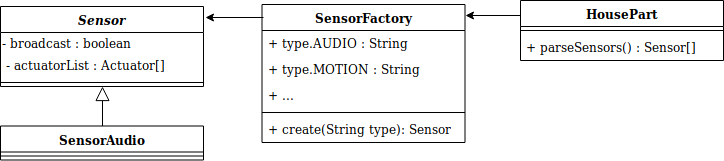
\includegraphics[width=\textwidth]{sensorfactory.png}
      \end{figure}
      \begin{minted}[autogobble]{java}
      public static Sensor create(String type, boolean broadcast){
        switch (type){
            case Sensor.AUDIO:
                return new SensorAudio(broadcast);
            ...
            default:
                return new SensorNull();
        }
      \end{minted}

      \subsection{Null Object}
        When parsing controllers, we don't null erroneous controllers. Instead, we assign them a default \texttt{SensorNull} type. This allows to lighten the code by not having to heavily charge the code with defensive measures against wrong configurations that could not be parsed. The Null Object will be an object of the same type as his parent, but will fail quietly (simply by doing nothing) instead of throwing a \texttt{NullPointerException}.
        \begin{figure}[!h]
          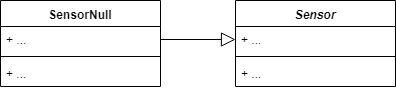
\includegraphics[scale=0.75]{nullsensor.png}
        \end{figure}
        \begin{minted}[autogobble]{java}
        public static Sensor create(String type, boolean broadcast){
          switch (type){
              case Sensor.AUDIO:
                  return new SensorAudio(broadcast);
              case Sensor.BADGE:
                  return new SensorBadgeDetector(broadcast);
              ...
              default:
                  return new SensorNull();
          }
        }
        \end{minted}
      \subsection{Facade}
        The \texttt{HomeController} is a facade to the system. It means that as a programmer you could interact and integrate the home automation system without caring about the concrete implementation of the houseparts, the parsers, the sensor communications, ... This pattern is very often used in large systems with many objects within a configuration and is almost always implicitly used with large polymorphed implementations.
        
        \emph{Note that we don't put the class diagram here as the relevant part of the diagram is the entire implementation. Refer to the updated complete class diagram and note how you can interact with a single class to create the whole system.}

        \begin{minted}[autogobble]{java}
        public static void main (String[] args){
            myHouse = House.getOrCreate("src/config_big.json");
            if (args.length == 0) {
                scenario = new Scenario(myHouse);
                scenario.userInput();
            }
            else if (args.length == 1) {
                userInputScenario = false;
                scenario = new Scenario(myHouse, args[0]);
                scenario.fileInput();
            }
        }
        \end{minted}
      \subsection{Singleton}
        The \texttt{House} object is a singleton as the automation system would only need one house. We used a singleton because the system is heavily hierarchized (house, house part, sensors, actuators) and the house is central to it all. If you need to access another house part from the current one, you need to go back to the house object. Using a singleton ensures that we won't create a new object by mistake and we enforce the use of a single parent for the system hierarchy.

        \begin{figure}[!h]
          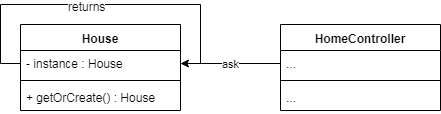
\includegraphics[scale=0.75]{singletonhouse.png}
        \end{figure}

        \begin{minted}[autogobble]{java}
        public class House{
          private House instance;
          public static House getOrCreate(String configFilename){
              ...
          }
          // Make constructor private to disable public/protected instanciation
          private House(String configFilename) {
            ...
          }
          ...
        }
        \end{minted}

      \subsection{Lesser patterns}
        Some patterns that are less relevant for this report were used. We can cite :
        \begin{description}
          \item [Builder] According to the documentation, the builder pattern is a way to create, step-by-step, large and complex objects composed of multiple smaller objects. That is essentially what the \texttt{House} and \texttt{HousePart} do with the parsing. But we did not use the structure the pattern describes so it is only a pseudo-builder.
          \item [Iterator] Natively implemented in Java, we loop over our objects with the \texttt{for each} java structure, which uses iterators.
          \item [Interpreter] Technically, the command line interpreter is an interpreter pattern as it translates human-readable commands to concrete system actions, but we feel the interpreter is not mature enough to be cited as a fully-implemented pattern.
          \item [Front Controller] \texttt{Scenario} is a singleton (static) class which handles the requests from multiple sources (file and user input), translates them to system functions (\texttt{FakeEvent}) and logs the results to the system output. Once again, this was not proposed as a fully-implemented pattern, because the class is mainly a dispatcher and not a logger per se (the application is single-threaded and uses the standard output).
        \end{description}
               
	\section{Conclusion}
		In this document, we presented and discussed the two extensions we implemented, that is the parametrization component and the command interpreter. We also reviewed the variability points of our program.
		Finally, we showed and discussed the design patterns we used throughout the code.
		
		In the appendices, you will find our class diagram and feature model. We updated them in accordance to the remarks we were given and the changes we made in our codde.

  \newpage
  \begin{appendices}
  	\section*{Appendices}
		You can find the updated UML diagram hereafter. The changes we made in our code can be seen on it.
		As last time, it is important to say that this diagram is highly conceptual, which means there are implementation specific details that are not represented. However, the main architecture is there.
		
		\begin{figure}[H]
			\centering
			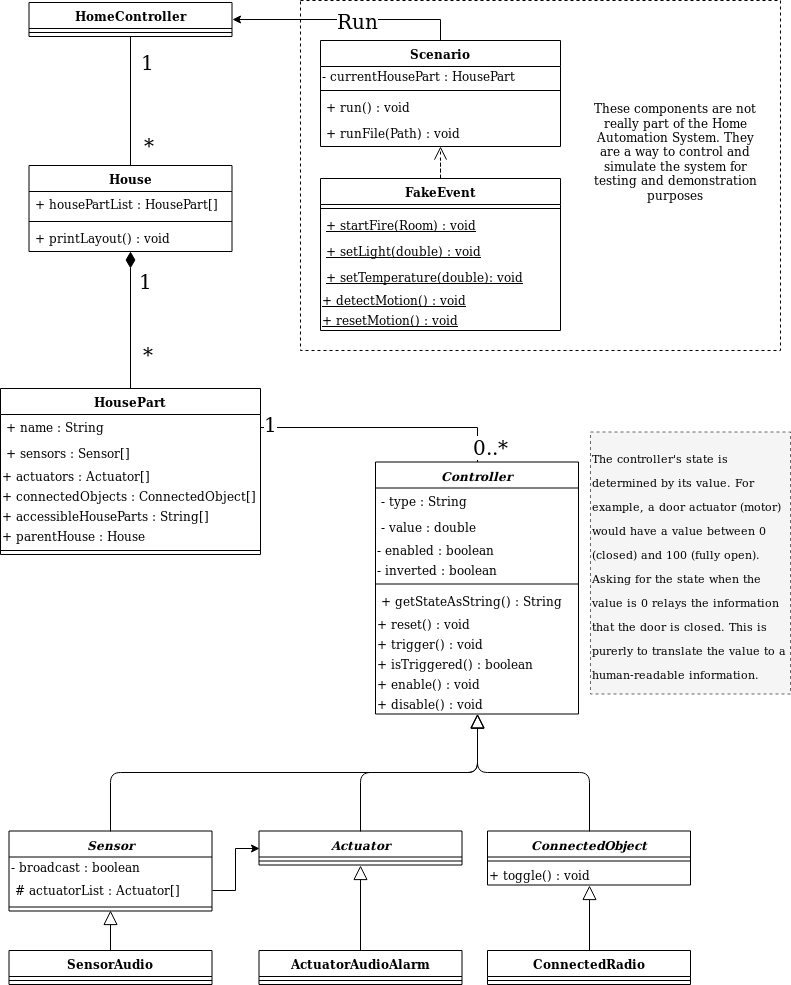
\includegraphics[scale=0.49]{UML-diagram_updated.png}
		\end{figure}
	
		Hereafter you will find the updated feature model.
	    \begin{changemargin}{-2cm}{-3cm}
    	  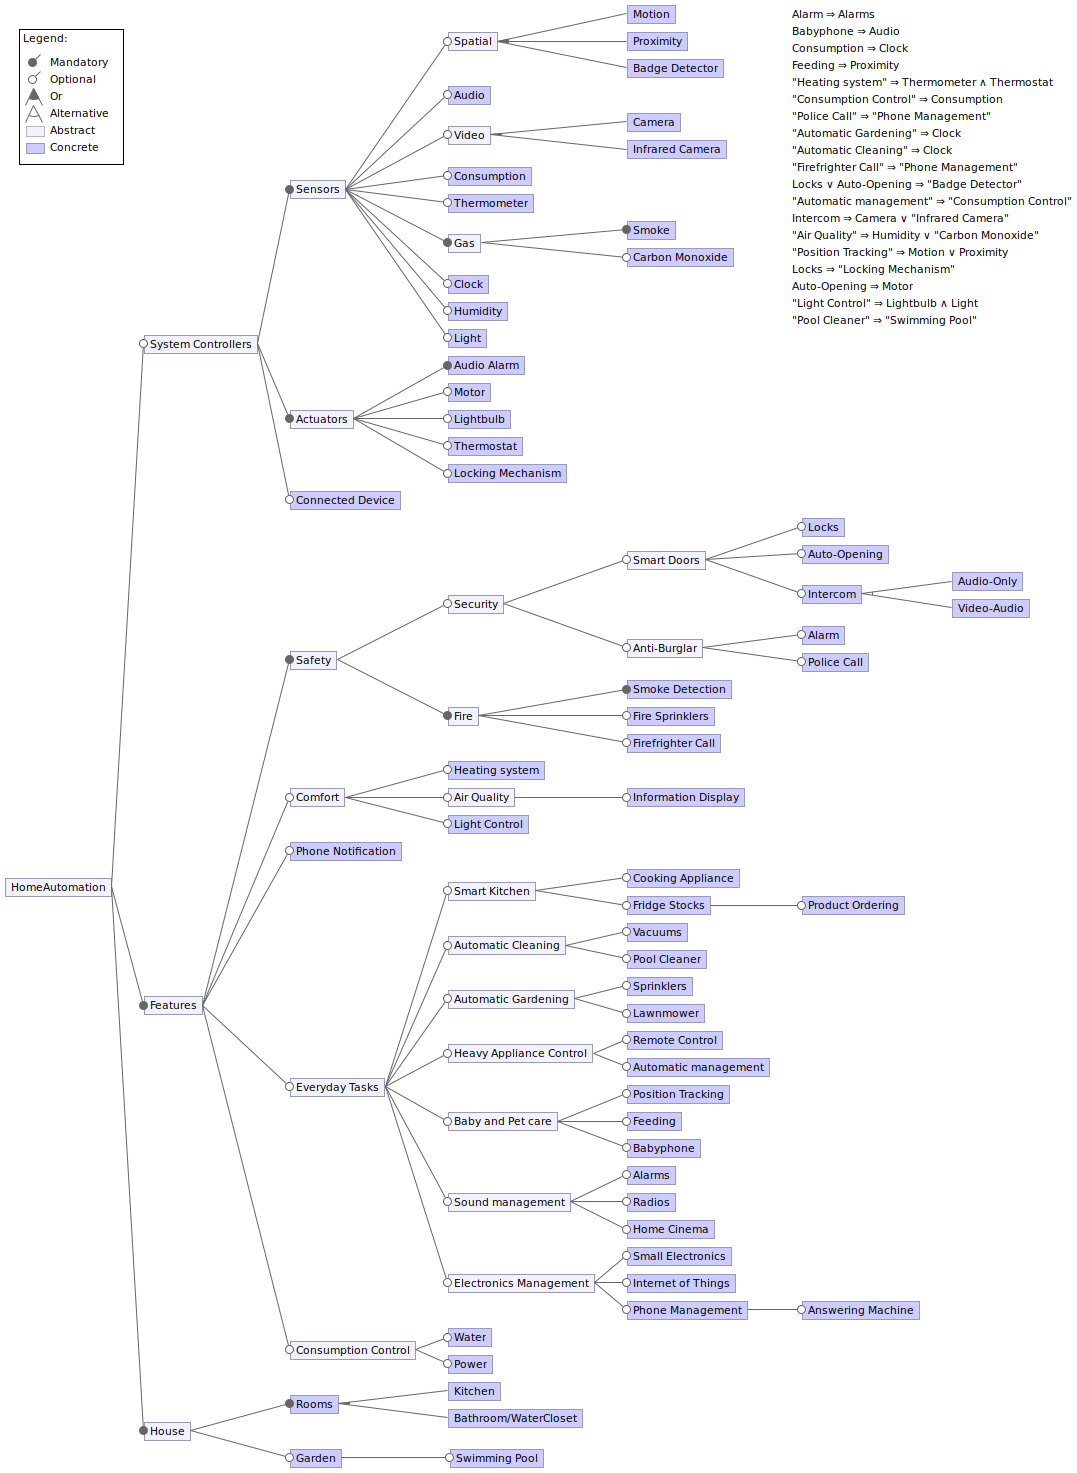
\includegraphics[width=\textwidth]{featuremodel_revisited}
	    \end{changemargin}
  \end{appendices}

\end{document}
